% defer/rcuintro.tex

\subsection{Introduction to RCU}
\label{sec:defer:Introduction to RCU}

앞의 섹션들에서 이야기된 방법들은 어느정도 확장성 있긴 했지만 모두 Pre-BSD
라우팅 테이블을 위한 성능에 있어서 이상적이지 못했습니다.
Pre-BSD 탐색 오버헤드가 싱글 쓰레드 탐색에서와 동일하게끔, 병렬로 수행되는
탐색이 싱글 쓰레드에서의 탐색과 동일한 어셈블리어 인스트럭션 시퀀스를
수행한다면 좋을 겁니다.
이는 좋은 목표가 될 수 있지만, 그러기 위해서는 구현 단계에서 많은 심각한 질문을
이끌어냅니다.
하지만 이걸 시도하면 어떤 일이 벌어질지 알아보고 삽입과 삭제를 구분해서
다뤄봅시다.
\iffalse

The approaches discussed in the preceding sections have provided
some scalability but decidedly non-ideal performance for the
Pre-BSD routing table.
It would be nice if the overhead of Pre-BSD lookups was the same as
that of a single-threaded lookup, so that the parallel lookups would
execute the same sequence of assembly language instructions as would a
single-threaded lookup.
Although this is a nice goal, it does raise some serious implementability
questions.
But let's see what happens if we try, treating insertion and deletion
separately.
\fi

\begin{figure}[tb]
\begin{center}
\resizebox{3in}{!}{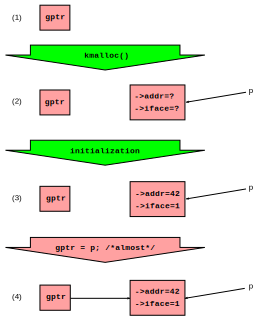
\includegraphics{defer/RCUListInsertClassic}}
\end{center}
\caption{Insertion With Concurrent Readers}
\label{fig:defer:Insertion With Concurrent Readers}
\end{figure}

아이템 추가를 위한 고전적인 방법이
Figure~\ref{fig:defer:Insertion With Concurrent Readers} 에 표현되어 있습니다.
첫번째 열은 기본 상태를 보이는데, \co{gptr} 은 \co{NULL} 값을 갖습니다.
두번째 열에서는 하나의 구조체를 메모리 할당하는데, 초기화 되지 않은 부분들은
물음표로 표시되어 있습니다.
세번째 열에서는 이 구조체를 초기화 시킵니다.
다음으로, \co{gptr} 이 이 새로운 원소를 가리키도록 그 값을
할당합니다.\footnote{
	많은 컴퓨터 시스템들에서, 컴파일러와 CPU가 간섭을 끼칠 수 있기 때문에
	단순한 값 할당은 충분하지 못합니다.
	이런 문제에 대해서는 Section~\ref{sec:defer:RCU Fundamentals} 에서
	다루게 될 겁니다.}
최근의 범용 시스템에서 이 값 할당은 어토믹해서 동시에 수행되는, 읽기를 하는
쓰레드들은 \co{NULL} 포인터 또는 새로운 구조체 \co{p} 로의 포인터 둘 중
하나만을 보게 되지, 두 값 중 일부가 합쳐져 있는 값은 보지 못합니다.
따라서, 각각의 읽기를 하는 쓰레드는 기본값인 \co{NULL} 을 보거나
기본값이 아닌 값을 보게 되거나일 것이며 어느 쪽이든 읽기는 일관적인 결과만을
보게 됨이 보장됩니다.
이뿐만이 아니라, 읽기를 수행하는 쓰레드는 다른 비싼 동기화 기능을 사용할 필요가
없어서, 이 방법은 리얼타임 쪽의 사용에 꽤 적합할 겁니다.\footnote{
	다시 말하지만, 많은 컴퓨터 시스템들에서 컴파일러와 DEC Alpha
	시스템에서라면 CPU가 간섭을 행하는 것을 막기 위한 추가 작업이
	필요합니다.
	이에 대해서는 Section~\ref{sec:defer:RCU Fundamentals} 에서
	이야기합니다.}
\iffalse

A classic approach for insertion is shown in
Figure~\ref{fig:defer:Insertion With Concurrent Readers}.
The first row shows the default state, with \co{gptr} equal to \co{NULL}.
In the second row, we have allocated a structure which is uninitialized,
as indicated by the question marks.
In the third row, we have initialized the structure.
Next, we assign \co{gptr} to reference this new element.\footnote{
	On many computer systems, simple assignment is insufficient
	due to interference from both the compiler and the CPU.
	These issues will be covered in
	Section~\ref{sec:defer:RCU Fundamentals}.}
On modern general-purpose systems, this assignment is atomic in the
sense that concurrent readers will see either a \co{NULL} pointer
or a pointer to the new structure \co{p}, but not some mash-up
containing bits from both values.
Each reader is therefore guaranteed to either get the
default value of \co{NULL} or to get the newly installed
non-default values, but either way each reader will see
a consistent result.
Even better, readers need not use any expensive synchronization
primitives, so this approach is quite suitable for real-time use.\footnote{
	Again, on many computer systems, additional work is required
	to prevent interference from the compiler, and, on DEC Alpha
	systems, the CPU as well.
	This will be covered in
	Section~\ref{sec:defer:RCU Fundamentals}.}
\fi

\begin{figure}[tb]
\begin{center}
\resizebox{3in}{!}{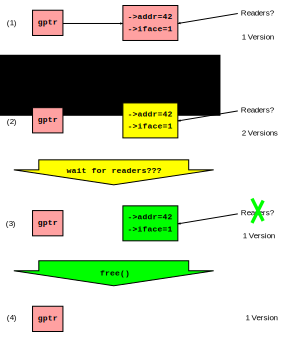
\includegraphics{defer/RCUListDeleteClassic}}
\end{center}
\caption{Deletion From Linked List With Concurrent Readers}
\label{fig:defer:Deletion From Linked List With Concurrent Readers}
\end{figure}

하지만 동시에 읽기 쓰레드에 의해 레퍼런스 되고 있는 데이터는 언젠가는 없어져야
할 겁니다.
Figure~\ref{fig:defer:Deletion From Linked List With Concurrent Readers} 와
같이 링크드 리스트에서 원소를 삭제하는, 더 복잡한 예제를 봅시다.
이 리스트는 초기에 원소~\co{A}, \co{B}, 그리고 \co{C} 를 가지고 있으며, 여기서
원소~\co{B} 를 삭제해야 합니다.
먼저 \co{list_del()} 을 사용해 삭제를 진행하는데,\footnote{
	역시 앞서 말했듯 이는 추상화된 예이고,
	Section~\ref{sec:defer:RCU Fundamentals} 에서 이에 관련해서 더 이야기
합니다.}
모든 새로운 읽기 쓰레드들은 원소~\co{B} 를 리스트에서 삭제된
것으로 보게 될 겁니다.
하지만, 이 원소를 여전히 보고 있는 오래된 읽기 쓰레드들도 있을 수
있습니다.
이 오래된 읽기 쓰레드들이 종료되고 나면, 원소~\co{B} 를 안전히 메모리
해제시켜서 그림의 아래쪽에 그려진 상태를 만들 수 있을 겁니다.
\iffalse

But sooner or later, it will be necessary to remove data that is
being referenced by concurrent readers.
Let us move to a more complex example where we are removing an element
from a linked list, as shown in
Figure~\ref{fig:defer:Deletion From Linked List With Concurrent Readers}.
This list initially contains elements~\co{A}, \co{B}, and \co{C},
and we need to remove element~\co{B}.
First, we use \co{list_del()} to carry out the removal,\footnote{
	And yet again, this approximates reality, which will be expanded
	on in Section~\ref{sec:defer:RCU Fundamentals}.}
at which point all new readers will see element~\co{B} as having been
deleted from the list.
However, there might be old readers still referencing this element.
Once all these old readers have finished, we can safely free
element~\co{B}, resulting in the situation shown at the bottom of
the figure.
\fi

하지만, 그 종료 시점을 어떻게 알까요?

레퍼런스 카운팅 방법의 경우는,
Chapter~\ref{chp:Counting} 의
Figure~\ref{fig:count:Atomic Increment Scalability on Nehalem}
가 락킹과 시퀀스 락킹처럼 긴
딜레이를 가져올 수 있음을 보이므로 어렵습니다.

읽기 쓰레드들이 그 존재를 알리기 위한 일을 전혀 안하는,
극단적인 상황을 생각해 봅시다.
이는 읽기 쓰레드들에 최적의 성능을 가능하게 하겠지만
(아무것도 안해도 되니까요), 업데이트
쓰레드는 어떻게 모든 예전 읽기 쓰레드들의 종료를 알지에 대한 질문이
남습니다.
여기에 합리적 답을 하기 위해서는 추가적인 제약이 분명
필요합니다.
\iffalse

But how can we tell when the readers are finished?

It is tempting to consider a reference-counting scheme, but
Figure~\ref{fig:count:Atomic Increment Scalability on Nehalem}
in
Chapter~\ref{chp:Counting}
shows that this can also result in long delays, just as can
the locking and sequence-locking approaches that we already rejected.

Let's consider the logical extreme where the readers do absolutely
nothing to announce their presence.
This approach clearly allows optimal performance for readers
(after all, free is a very good price),
but leaves open the question of how the updater can possibly
determine when all the old readers are done.
We clearly need some additional constraints if we are to provide
a reasonable answer to this question.
\fi

일부 운영체제에 적합한 제약은 쓰레드가 CPU 를
빼앗기지 않는 상황 (non-preemptible) 입니다.
CPU 를 빼앗길 수 없는 환경에서 쓰레드는 명시적이고 자발적으로
블락킹 되기 전까지는 수행을 계속합니다.
즉, 블락킹 없이 반복되는 무한루프는 CPU 를
무한루프 이외의 목적으로는 사용될 수 없게 하다는 의미입니다.\footnote{
	반면, CPU 를 빼앗길 수 있는 환경에서의 무한루프는 여전히 CPU 시간을
	낭비하고 있긴 하지만, 이 CPU 는 다른 일을 할 수 있을 겁니다.}
CPU 를 뺏길 수 없다는 특성은 또한 쓰레드들이 스핀락을 잡고 있는 동안은 블락킹
되지 않아야 할 것을 필요로 합니다.
이런 금지사항이 없다면, 블락된 쓰레드에 의해 잡혀 있는 스핀락을 획득하려
시도하며 루프를 도는 쓰레드들에 의해 모든 CPU 가 소모되게 될수도 있습니다.
루프를 도는 쓰레드들은 락을 잡기 전까지는 자신들의 CPU 들을 놓지 않을 것인데,
락을 잡고 있는 쓰레드는 이 루프를 돌고 있는 쓰레드들이 CPU 를 놓기 전까지는 그
락을 놓을 수가 없습니다.
이는 고전적인 deadlock 상황입니다.
\iffalse
One constraint that fits well with some operating-system kernels is to
consider the case where threads are not subject to preemption.
In such non-preemptible environments, each thread runs until it
explicitly and voluntarily blocks.
This means that an infinite loop without blocking will render a CPU
useless for any other purpose from the start of the infinite loop
onwards.\footnote{
	In contrast, an infinite loop in a preemptible environment
	might be preempted.
	This infinite loop might still waste considerable CPU time,
	but the CPU in question would nevertheless be able to do
	other work.}
Non-preemptibility also requires that threads be prohibited from blocking
while holding spinlocks.
Without this prohibition, all CPUs might be consumed by threads
spinning attempting to acquire a spinlock held by a blocked thread.
The spinning threads will not relinquish their CPUs until they acquire
the lock, but the thread holding the lock cannot possibly release it
until one of the spinning threads relinquishes a CPU.
This is a classic deadlock situation.
\fi

이와 똑같은 제약사항을 링크드 리스트를 횡단하며 읽기를 하는 쓰레드들에도
가해봅시다: 그런 쓰레드들은 리스트 횡단이 완료되기 전까지는 블락되는 것이
허용되지 않습니다.
업데이트 쓰레드가 \co{list_del()} 을 실행 완료한 직후인
Figure~\ref{fig:defer:Deletion From Linked List With Concurrent Readers} 의
두번째 줄로 돌아가서, CPU~0 가 컨텍스트 스위칭을 한다고 생각해 봅시다.
읽기 쓰레드들은 링크드 리스트 횡단 중에 블락되는 것은 허용되지 않으므로, CPU~0
에서 수행되던 모든 시간상 앞의 읽기 쓰레드들은 완료되었음이 보장됩니다.
이 이야기를 다른 CPU 들에도 적용해 보자면, 각 CPU 가 일단 컨텍스트 스위칭이
수행됨을 확인했다면, 모든 시간상 앞의 읽기 쓰레드들은 완료되었고, 더이상
원소~\co{B} 를 레퍼런스 하고 있는 읽기 쓰레드는 더이상 없다고 보장된다고 볼 수
있습니다.
그렇다면 업데이트 쓰레드는 안전하게 원소~\co{B} 를 메모리 해제해서
Figure~\ref{fig:defer:Deletion From Linked List With Concurrent Readers} 의
가장 아래의 상태를 만들어낼 수 있습니다.
\iffalse

Let us impose this same constraint on reader threads traversing the
linked list: such threads are not allowed to block until after
completing their traversal.
Returning to the second row of
Figure~\ref{fig:defer:Deletion From Linked List With Concurrent Readers},
where the updater has just completed executing \co{list_del()},
imagine that CPU~0 executes a context switch.
Because readers are not permitted to block while traversing the linked
list, we are guaranteed that all prior readers that might have been running on
CPU~0 will have completed.
Extending this line of reasoning to the other CPUs, once each CPU has
been observed executing a context switch, we are guaranteed that all
prior readers have completed, and that there are no longer any reader
threads referencing element~\co{B}.
The updater can then safely free element~\co{B}, resulting in the
state shown at the bottom of
Figure~\ref{fig:defer:Deletion From Linked List With Concurrent Readers}.
\fi

\begin{figure}[tb]
\centering
\resizebox{3in}{!}{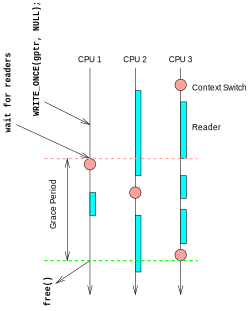
\includegraphics{defer/QSBRGracePeriod}}
\caption{RCU QSBR: Waiting for Pre-Existing Readers}
\label{fig:defer:RCU QSBR: Waiting for Pre-Existing Readers}
\end{figure}

이런 방법은 \emph{quiescent state based
reclamation}(QSBR)~\cite{ThomasEHart2006a} 이라 명명되어 있습니다.
하나의 QSBR 방법이
Figure~\ref{fig:defer:RCU QSBR: Waiting for Pre-Existing Readers},
에 그림의 꼭대기부터
바닥까지로 시간의 흐름에 따라 그려져 있습니다.

이런 방법의 상품 품질 구현은 상당히 복잡할 수 있지만, 장난감 수준 구현은 상당히
간단합니다:
\iffalse

This approach is termed \emph{quiescent state based reclamation}
(QSBR)~\cite{ThomasEHart2006a}.
A QSBR schematic is shown in
Figure~\ref{fig:defer:RCU QSBR: Waiting for Pre-Existing Readers},
with time advancing from the top of the figure to the bottom.

Although production-quality implementations of this approach can be
quite complex, a toy implementation is exceedingly simple:
\fi

\vspace{5pt}
\begin{minipage}[t]{\columnwidth}
\scriptsize
\begin{verbatim}
  1 for_each_online_cpu(cpu)
  2   run_on(cpu);
\end{verbatim}
\end{minipage}
\vspace{5pt}

이 \co{for_each_online_cpu()} 함수는 모든 CPU 들에 루프를 돌고, \co{run_on()}
함수는 현재 쓰레드가 특정 CPU 에서 수행되게 해서 목적지 CPU 가 컨텍스트
스위칭을 수행하게 만듭니다.
따라서, 일단 한번 \co{for_each_online_cpu()} 가 완료되면, 각 CPU 는 컨텍스트
스위치를 수행한 것이고, 따라서 모든 시간상 앞의 읽기 쓰레드들은 완료되었음이
보장됩니다.
\iffalse

The \co{for_each_online_cpu()} primitive iterates over all CPUs, and
the \co{run_on()} function causes the current thread to execute on the
specified CPU, which forces the destination CPU to execute a context
switch.
Therefore, once the \co{for_each_online_cpu()} has completed, each CPU
has executed a context switch, which in turn guarantees that
all pre-existing reader threads have completed.
\fi

이 방법은 상품 수준의 품질이 \emph{아님} 을 알아 두시기 바랍니다.
여러개의 일반적이지 않은 문제 경우의 처리와 여러개의 강력한 최적화의 필요성은
상품 수준 품질의 구현은 상당한 추가적 복잡도를 의미합니다.
또한, CPU 강탈이 가능한 환경에서의 RCU 구현은 읽기 쓰레드들이 실제로 뭔가를
할것을 필요로 합니다.
하지만, 이 간단한 CPU 강탈 불가한 상황의 접근법은 개념적으로는 완벽하고, 다음
섹션에서 다루어질 RCU 의 기본을 이해하기 위한 좋은 초기 토대가 될겁니다.
\iffalse

Please note that this approach is \emph{not} production quality.
Correct handling of a number of corner cases and the need for a number
of powerful optimizations mean that production-quality implementations
have significant additional complexity.
In addition, RCU implementations for preemptible environments
require that readers actually do something.
However, this simple non-preemptible approach is conceptually complete,
and forms a good initial basis for understanding the RCU fundamentals
covered in the following section.
\fi
